\documentclass[tikz,crop]{standalone}

\usepackage{tikz}
\usepackage{physics}
\usetikzlibrary{hobby}  



%------------   Todo está en 2D porque no entiendo 3D   :c    ------------%


\begin{document}

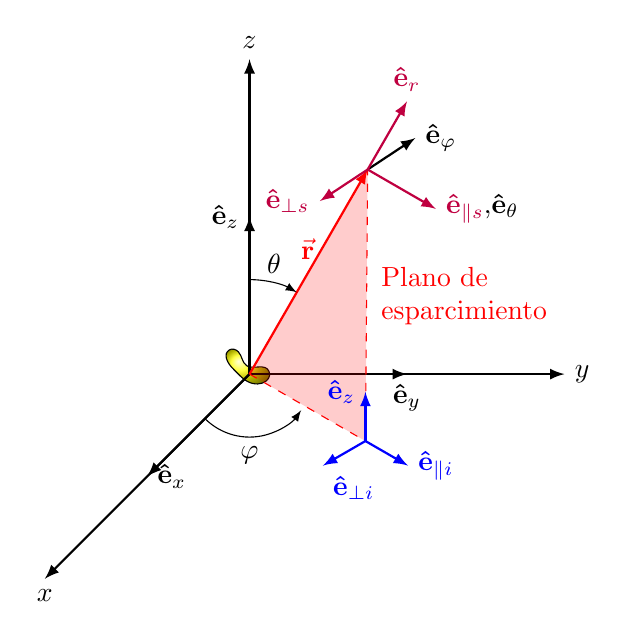
\begin{tikzpicture}[scale=1]

\coordinate (O) at (0,0);

%------------------------------------------------------- Particle
\shade[draw,use Hobby shortcut,closed=true, ball color=yellow, rotate=45]
(.2,-.15) .. (.05,.1) .. (.1,.3) .. (.03,.4) .. (-.1,.2) .. (-.1,.05);

%------------------------------------------------------- Coordinate system axes
\draw[thick,- latex] (O) -- (-2.6,-2.6) node[anchor=north ]{$x$};
\draw[thick,- latex] (O) -- (4,0) node[anchor= west]{$y$};
\draw[thick,- latex] (O) -- (0,4) node[anchor=south]{$z$};

%------------------------------------------------------- Cartesian vectors
\draw[thick,- latex] (O) -- (-1.3,-1.3) node[anchor=west ]{$\vu{e}_x$};
\draw[thick,- latex] (O) -- (2,0) node[anchor= north]{$\vu{e}_y$};
\draw[thick,- latex] (O) -- (0,2) node[anchor=east]{$\vu{e}_z$};

%------------------------------------------------------- polar variables
\draw[thick,red,- latex] (O) -- (60:3); \node at (65:1.75) {\color{red} $\va{r}$}; 

\path (O)++(90-15:1.2)node[anchor=south]{$\theta$};    
\draw[- latex](90:1.2)arc(90:60:1.2);

\path (O)++(-90:.8)node[anchor=north ]{$\varphi$};    
\draw[- latex](-135:.8)arc(-135:-35:.8);
	
%------------------------------------------------------- Scattering plane

\draw[-, dashed,red] (O) -- (-30:1.7);		%xy proyection
\draw[-,dashed,red] (-30:1.7) -- (60:3) ;	%normal proyection
\fill[red,opacity=.2] (O)-- (-30:1.7)--(60:3)--(O);  %Shade
\node at (20:2.9) [ align=left, red]{ Plano de\\ esparcimiento};
	
%------------------------------------------------------- Top Vector
\begin{scope}[shift = (60:3), rotate=-30, scale = .5]
\draw[thick,- latex, purple] (0,0) -- (-.65,-1.3) node[anchor= east ]{$\vu{e}_{\perp s}$};
\draw[thick,- latex] (0,0) -- (.65,1.3) node[anchor=west ]{$\vu{e}_\varphi$};
\draw[thick,- latex, purple] (0,0) -- (2,0) node[anchor= west]{$\vu{e}_{\parallel s}${\color{black},$\vu{e}_\theta$}};
\draw[thick,- latex, purple] (0,0) -- (0,2) node[anchor=south]{$\vu{e}_r$};
\end{scope}	

%------------------------------------------------------- Bottom Vectors
\begin{scope}[shift = (-30:1.7), rotate=-30, scale = .5]
\draw[thick,- latex, blue] (0,0) -- (90+30:1.25) node[anchor=east]{$\vu{e}_z$};
\draw[thick, blue ,- latex] (0,0) -- (-120:1.25) node[anchor=north west]{$\vu{e}_{\perp i}$};
\draw[thick,blue, - latex] (0,0) -- (1.25,0) node[anchor= west]{$\vu{e}_{\parallel i}$};
\end{scope}	

\end{tikzpicture}


\end{document}
